\documentclass[10pt]{article}

\usepackage[paperwidth=19.05cm,paperheight=26.00cm,top=1.65cm,bottom=1.80cm,left=1.55cm,right=1.55cm]{geometry}
\usepackage[T1]{fontenc}
\usepackage[utf8]{inputenc}
\usepackage{mathptmx}
\usepackage{graphicx}
\usepackage{amsmath}
\usepackage{array}
\usepackage{booktabs}
\usepackage{longtable}
\usepackage{tabularx}
\usepackage{ragged2e}
\usepackage{enumitem}
\usepackage{caption}
\usepackage{fancyhdr}
\usepackage{titlesec}
\usepackage[hidelinks]{hyperref}

\setlength{\parindent}{0pt}
\setlength{\parskip}{6pt}
\setlength{\headheight}{14pt}
\captionsetup{font=small,labelfont=bf,labelsep=colon}
\renewcommand{\arraystretch}{1.16}
\newcolumntype{Y}{>{\RaggedRight\arraybackslash}X}
\newcolumntype{P}[1]{>{\RaggedRight\arraybackslash}p{#1}}

\titleformat{\section}{\normalfont\large\bfseries}{\thesection.}{0.5em}{}
\titleformat{\subsection}{\normalfont\normalsize\bfseries}{\thesubsection}{0.5em}{}
\titleformat{\subsubsection}{\normalfont\normalsize\itshape}{\thesubsubsection}{0.5em}{}
\titlespacing*{\section}{0pt}{10pt}{4pt}
\titlespacing*{\subsection}{0pt}{8pt}{3pt}
\titlespacing*{\subsubsection}{0pt}{7pt}{2pt}

\pagestyle{fancy}
\fancyhf{}
\fancyhead[L]{\footnotesize Navya Sharma / Procedia Computer Science 00 (2026) 000--000}
\fancyhead[R]{\footnotesize \thepage}
\renewcommand{\headrulewidth}{0pt}

\begin{document}

\thispagestyle{empty}
\begin{center}
{\small Available online at www.sciencedirect.com\par}
{\LARGE ScienceDirect\par}
{\small Procedia Computer Science 00 (2026) 000--000\par}
\vspace{4pt}
{\small www.elsevier.com/locate/procedia\par}
\vspace{12pt}
{\small International Conference on Machine Learning and Data Engineering (ICMLDE 2023)\par}
\vspace{14pt}
{\Large\bfseries GraphRAG-Based Research Paper Assistant for Multi-Paper Knowledge Synthesis\par}
\vspace{10pt}
{\normalsize Navya Sharma\par}
\vspace{5pt}
{\small Department of Information Technology, Bharati Vidyapeeth College of Engineering, Paschim Vihar, New Delhi\par}
{\small E-mail address: navyasharma.1307@gmail.com\par}
\end{center}

\vspace{8pt}
\textbf{Abstract}\par
In the past few years, we have seen an increase in the quantity of research papers being published all over the world in various different domains such as Artificial Intelligence, Data Science and Cyber Security. While they offer a lot of insight, reading and understanding research papers can be time consuming and requires a lot of manual effort. A lot of tools exist specifically targeting research paper but they only deal with summarization of one paper and do not compare how multiple papers are connected with one another and do not offer deeper reasoning. In order to address this gap, GraphRAG based research paper analyser was proposed in which semantic reasoning would be combined with structured knowledge representation.

The system implements several important features which aims to simplify multi paper analysis. Firstly, a paper summarizer was implemented which provides detailed analysis including problem definition, methodology, results, limitations, and research gaps, helping users understand papers in a more comprehensive and organized manner. A chatbot is also implemented which combines both contextual and structural reasoning to give intelligent answers. Additionally, research paper recommendation and comparison features are established using a hybrid similarity model that combines embedding similarity with entity overlap which in turn helps provide interpretable explanations using shared methods, dataset and topics. Lastly clustering is done so that visualization of research papers become easier and the users can easily analyse papers of the same and different domains and their features. The hybrid model achieves a significant improvement of 11.53\% in comparing same domain papers which further proves the significance of using hybrid model. One of the major features of this model is its explainability i.e. it is able to provide concrete proof as to why papers are similarly ranked rather than just depending on vector embeddings and 100\% explainability was achieved.

\textbf{Keywords:} GraphRAG; Knowledge Graph; Research Paper Summarization; Semantic Search; Retrieval-Augmented Generation; Multi-Paper Analysis

\section{Introduction}
With the recent advancements all over the world in various different fields, staying up to date has become the norm in the industry and people are expected to have a knowledge of everything that is new in the market. The best way to stay up to date is by reading research papers. While they provide intensive knowledge regarding any topic, they can be too cumbersome to read and analysing how one research paper is different from the other can be difficult. Existing technologies focus on single paper summarization and analysis and do not consider multi paper analysis of same and different domains. Cosine similarity is traditionally used in the existing systems but they have a very big disadvantage when analysing research papers. It often assigns high similarity score to papers who are semantically similar even when they belong to different domains. This happens because cosine similarity relies only on vector representations and does not consider the underlying structure of the document. So in order to overcome this problem, a hybrid system was established combining semantic retrieval with GraphRAG based structural reasoning.

This allows the system to not only identify related and unrelated papers more reliably but also provide reasoning as to why it came to that conclusion, making it more suitable for multi-paper analysis compared to purely embedding based approaches. This makes the system more trustworthy as GraphRAG shows the shared entities between different research papers such as common methods, datasets or models. It makes the system more transparent compared to black box embedding methods. The aim of this project is to simplify and streamline the process of literature review by providing an intelligent assistant that supports faster understanding, comparison, and knowledge discovery from academic papers.

\begin{figure}[htbp]
\centering
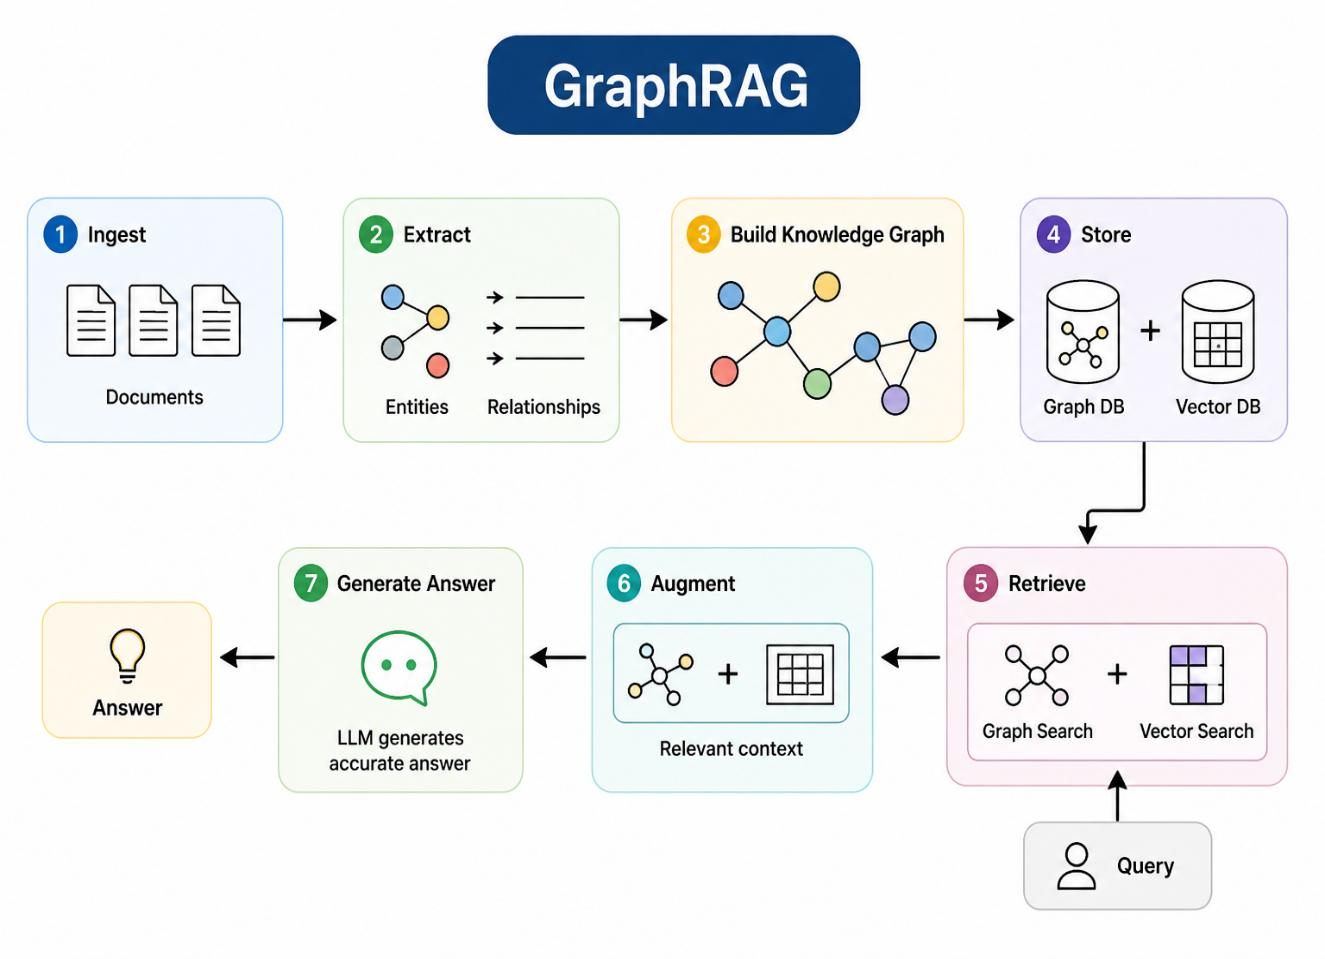
\includegraphics[width=0.78\linewidth]{paper_figures/figure1_graphrag.jpeg}
\caption{GraphRAG}
\label{fig:graphrag}
\end{figure}

\begin{figure}[htbp]
\centering
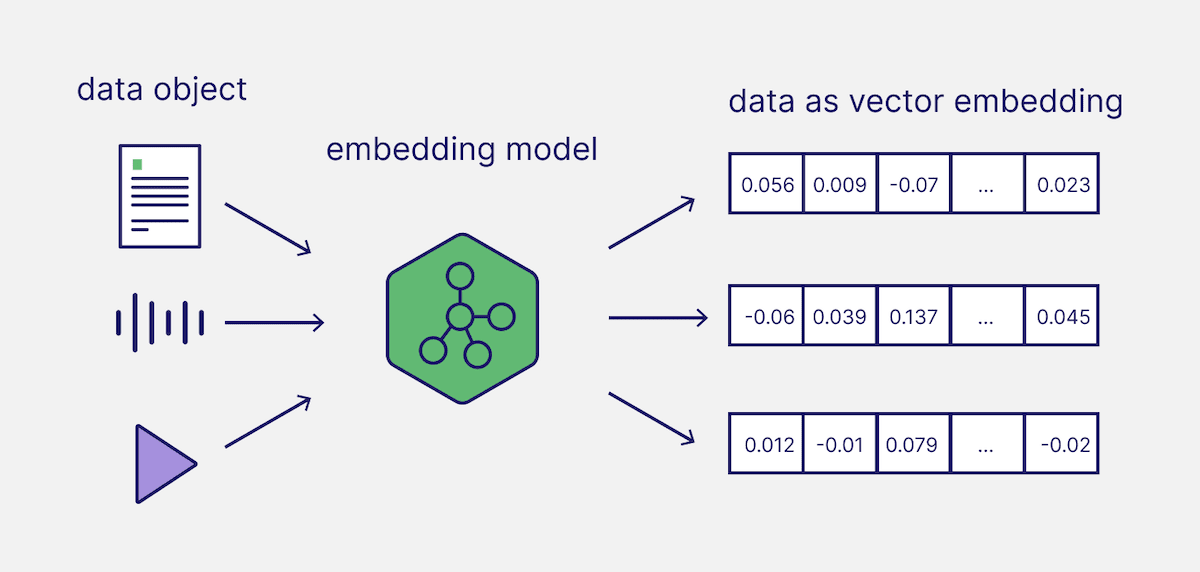
\includegraphics[width=0.78\linewidth]{paper_figures/figure2_vector_embeddings.png}
\caption{Vector Embeddings}
\label{fig:vector-embeddings}
\end{figure}

\section{Related Work}
Various techniques have been developed all over the world to improve and work upon information retrieval, knowledge extraction, and multi document understanding. The key contributions are discussed below.

Lewis et al. [1] was responsible for introducing the concept of Retrieval Augmented Generation (RAG) where existing documents are retrieved using similarity search and then answers are generated based on this. While it does provide accuracy, it fails to capture relationships between different documents. In order to further improve upon the work of Lewis, Karpukhin et al. [9] made a Dense Passage Retrieval (DPR), which uses dense embeddings instead of simple keyword matching making it more reliable. This has become the foundation of the modern retrieval systems today. However the major disadvantage of both RAG and DPR was that it only considered semantic meaning and failed to capture relation between different documents. So Edge et al. [2] introduced GraphRAG, which helps identify relationships and extracts entities to build graph and generate answers with structured reasoning. Zhang et al. [3] also carried forward the work done by Edge et al. and categorised GraphRAG methods into knowledge-based, index-based, and hybrid types to prove how graphs are needed for reasoning and complex queries. Similarly, Knollmeyer et al. [4] extended this idea by integrating documents level knowledge graphs into the RAG pipeline, where entities and relationships were extracted from the document to build knowledge graphs which helped improve retrieval accuracy. Etzioni et al. [5] was responsible for exploring rule based and pattern based extraction which laid the foundation for later works. Later, Bordes et al. [12] was responsible for introducing translational embedding models (TransE) which led to efficient representation of entity relationships.

Yates et al. [6] proposed Open Information Extraction, a method that extracts relationships from text in the form of triples (subject, relation, object). This helps in converting unstructured text into structured knowledge which can be later used to build knowledge graphs. Sentence BERT developed by Reimers and Gurevych [10], have improved semantic search by doing sentence embeddings which are much more useful in large documents and are widely used now in vector databases. Gao et al. [7] investigated existing RAG systems and strategies and how there is a need for structural reasoning in multi paper analysis and not just semantic retrieval. Wang et al. [8] was responsible for introducing hierarchical retrieval in documents where the structure of document is extracted along with semantic meaning to give better reasoning. Additionally, Devlin et al. [13] introduced BERT (Bidirectional Encoder Representations from Transformers), a transformer model which provides contextual understanding useful for Natural language processing, text summarization and text classification tasks. Graph based learning methods such as Graph Neural Networks (GNNs) was introduced by Wu et al. [15] which further improved upon the graph retrieval methods. Johnson et al. [14] also contributed to large scale similarity search by introducing efficient vector indexing techniques which enabled fast retrieval in high dimensional space making it essential for real time applications. Despite these advancements, still a large gap exists in multi paper reasoning and most systems focus on individual document rather than treating them as a structured unit. So there is a need to combine Graph based and Semantic retrieval to do multi paper analysis.

\begin{longtable}{P{2.1cm} P{2.1cm} P{2.2cm} P{2.9cm} P{5.0cm}}
\caption{Findings}\label{tab:findings}\\
\toprule
\textbf{Author and Year} & \textbf{Technique} & \textbf{Dataset / Application} & \textbf{Comparison / Focus} & \textbf{Remarks}\\
\midrule
\endfirsthead
\toprule
\textbf{Author and Year} & \textbf{Technique} & \textbf{Dataset / Application} & \textbf{Comparison / Focus} & \textbf{Remarks}\\
\midrule
\endhead
Lewis et al. (2020) [1] & Retrieval Augmented Generation (RAG) & Large text corpora & Compared with traditional LMs without retrieval & Introduces RAG but does not consider multi paper reasoning\\
Edge et al. (2024) [2] & GraphRAG & Large document collections & Compared with vector based RAG & Extracts entities and builds knowledge graphs which makes reasoning more structured\\
Zhang et al. (2025) [3] & GraphRAG Survey and Taxonomy & Various GraphRAG frameworks & Categorization of GraphRAG approaches & Mainly focuses on categorizing GraphRAG approaches and shows why graph based retrieval is useful\\
Knollmeyer et al. (2025) [4] & Document GraphRAG & SQuAD, HotpotQA & Compared with naive RAG & Shows improvement in retrieval accuracy, especially for multistep reasoning tasks\\
Etzioni et al. (2004) [5] & Knowledge Graph Construction & Web corpora & Pattern based extraction methods & Early work that set the base for pattern and rule-based extraction methods\\
Yates et al. (2007) [6] & Open Information Extraction (OpenIE) & Web scale text & Compared with traditional IE methods & Introduced extraction in the form of triples i.e. subject, relation and object\\
Gao et al. (2023) [7] & Advanced RAG Retrieval Strategies & QA datasets & Compared with standard vector retrieval & Points out the limitations of using only vector based retrieval methods\\
Wang et al. (2023) [8] & Hierarchical Retrieval & Large document repositories & Compared with flat retrieval & Uses hierarchical retrieval of documents which leads to structured extraction\\
Karpukhin et al. (2020) [9] & Dense Passage Retrieval (DPR) & Open-domain QA datasets & Dense vs sparse retrieval & DPR uses dense embedding instead of simple keyword matching making it more reliable\\
Reimers \& Gurevych (2019) [10] & Sentence BERT & Sentence similarity tasks & Compared with BERT embeddings & Proposes sentence level embeddings which is much better for similarity retrieval tasks\\
Hamilton et al. (2017) [11] & GraphSAGE (Graph Embeddings) & Large scale graph datasets & Inductive graph learning & Responsible for scalable learning proving efficient for large documents\\
Bordes et al. (2013) [12] & TransE (Knowledge Graph Embeddings) & Multi relational data & Compared with traditional KG models & Provides improved representation of entities and their relations\\
Devlin et al. (2019) [13] & BERT & NLP benchmarks (GLUE, SQuAD) & Pre trained transformer models & Transformer model which improves Natural language processing\\
Johnson et al. (2019) [14] & FAISS / Vector Search Optimization & Billion scale vector datasets & GPU based similarity search & Vector Indexing is done to improve retrieval speed in high dimensional space\\
Wu et al. (2021) [15] & Graph Neural Networks (GNNs) Survey & Graph based applications & Overview of GNN models & Gives an overview of GNN models and shows how they help in reasoning over graph data\\
Vaswani et al. (2017) [16] & Transformer (Attention Mechanism) & Machine translation datasets & Compared with RNNs and LSTMs & Introduces attention-based architecture which improves sequence modeling and forms the base of modern LLMs\\
Brown et al. (2020) [17] & GPT-3 (Large Language Model) & Multi-domain text datasets & Few-shot vs traditional supervised models & Demonstrates strong few-shot learning capability and scalability of large language models\\
Radford et al. (2019) [18] & GPT-2 (Generative Language Model) & Web text corpus & Compared with task-specific models & Shows that large-scale pretraining can perform multiple NLP tasks without fine-tuning\\
Raffel et al. (2020) [19] & T5 (Text-to-Text Transformer) & Colossal Clean Crawled Corpus (C4) & Unified framework for NLP tasks & Proposes converting all NLP tasks into a text-to-text format improving transfer learning\\
Guu et al. (2020) [20] & REALM (Retrieval-Augmented Language Model) & Wikipedia corpus & Compared with standard language models & Integrates retrieval into pretraining to improve knowledge-intensive task performance\\
\bottomrule
\end{longtable}

\section{Research Gap}
There have been significant improvements all over the world from Retrieval-Augmented Generation to Dense Passage Retrieval and GraphRAG-based systems. Still a lot of limitations exist specifically in the domain of research paper analysis. Most existing systems focus on single paper analysis without providing any option to do multi paper reasoning and view various different papers as a connected knowledge unit. This limits the users to perform comparative analysis of paper and how different papers improved on the work of previous papers. Another drawback is the lack of explainability of the retrieval systems i.e. they behave like black boxes and they often lack reasoning and justification of the answer they gave making them less trustworthy of academic use. One of the major problems in existing systems is that they assign higher similarity score for papers belonging to different domains because of the generic words used such as dataset, model etc. ignoring the actual concept. Even advanced RAG systems fail to capture explicit relationships such as shared methods, datasets, and models which are critical in research paper comparison and reasoning. Therefore, there is a clear need for a hybrid system that combines semantic retrieval with structured knowledge graphs to enable accurate, explainable, and efficient multi-paper analysis and knowledge synthesis.

\section{Methodology}
\subsection{System Architecture Overview}
The proposed system is a GraphRAG system where both semantic search as well as structured reason is combined making it a hybrid model. Traditionally, vector embedding are mostly used to capture semantic similarity but this has a major drawback when structured reasoning is required. Particularly in research domain, where the same idea can be written using different terms or where relationships (like a method used on a dataset) are important. In order to overcome this limitation, a dual strategy is implemented where each paper is represented as:
\begin{itemize}[leftmargin=*,noitemsep]
\item a dense embedding vector capturing semantic meaning;
\item a node within a knowledge graph capturing explicit relationships.
\end{itemize}

Rather than treating these as independent units, graph score is used at every step of the system be it similarity computation, ranking recommendations or explainability. The system first looks for the knowledge graph to see how documents are connected with one another and then sees the semantic similarity. This aids in providing structured reasoning and helps boost explainability and logic of the system.

The architecture is organized into five functional layers:
\begin{itemize}[leftmargin=*,noitemsep]
\item Document ingestion and structuring;
\item Semantic embedding and vector storage;
\item Entity extraction and normalization;
\item Knowledge graph construction;
\item Hybrid retrieval and GraphRAG reasoning.
\end{itemize}

A key design decision is that graph signals are treated as primary evidence during reasoning, with embedding similarity acting as a complementary signal. The system first looks for the knowledge graph to see how documents are connected with one another and then sees the semantic similarity. This aids in providing structured reasoning and helps boost explainability and logic of the system.

\begin{figure}[htbp]
\centering
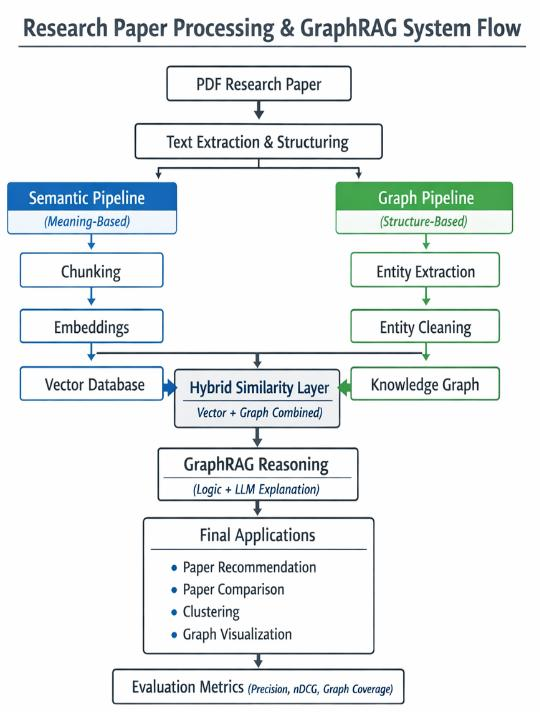
\includegraphics[width=0.62\linewidth]{paper_figures/figure3_system_flow.jpeg}
\caption{System Flow}
\label{fig:system-flow}
\end{figure}

\subsubsection{Document Ingestion and Structural Parsing}
The first step of the system is parsing the document in pdf format. In order to make a parsing tool which will consider different types of research paper formats also, a multi-stage parsing pipeline is employed to maximize robustness.

The extraction process proceeds in the following manner:
\begin{itemize}[leftmargin=*,noitemsep]
\item Layout-aware parsing using GROBID;
\item Heuristic extraction using pdfplumber;
\item Raw text fallback when structured parsing fails.
\end{itemize}

This approach ensures that pdf is properly extracted even when different formats exist. After extraction is done, the content is reorganised into a hierarchical format which preserves the actual structure of the document rather than flattening it into plain text so that the entities can be easily extracted. The following components are explicitly represented:
\begin{itemize}[leftmargin=*,noitemsep]
\item Abstract;
\item Section and subsection hierarchy;
\item Figures and tables (along with metadata if available);
\item Full text body.
\end{itemize}

Keeping the structure of the document has a lot of advantages particularly during the process of chunking and retrieval. As we maintain the context of the text due to the section headings, understanding context becomes easier which leads to more accurate and meaningful results. Another thing was observed that LLM processing to extract entities takes a lot of time, so a keyword-based entity extraction is also implemented to quickly identify basic entities such as methods, datasets, and models. Although this keyword based extraction is not as accurate as LLM results but this helps the system stay responsive and usable, even before the full processing is completed.

\subsubsection{Semantic Representation and Vector Storage}
Text is converted into embeddings using an embedding pipeline for similarity search. Instead of converting the entire document as a whole into vector embeddings, first the text is broken down into small chunks based on:
\begin{itemize}[leftmargin=*,noitemsep]
\item section boundaries as they help preserve context and meaning;
\item token-length constraints (to comply with model limits);
\item overlapping windows as they avoid loss of important information and helps to maintain continuity.
\end{itemize}

Each chunk is also stored along with metadata such as the paperID, section name, and the position of the text in the document. This helps in building a system which returns precise results.

The chunks are then encoded into dense vector representation using a transformer based embedding model i.e. bge-base-en-v1.5. This model produces high quality semantic embeddings which allows the system to capture the meaning of the text efficiently. These embeddings are then later used for similarity comparison and retrieval tasks.

The embeddings generated are then stored in the vector database Qdrant. This type of database supports fast similarity search using approximate nearest neighbour techniques. Qdrant also allows metadata based filtering which helps in extracting and narrowing down relevant chunks.

This layer is used for:
\begin{itemize}[leftmargin=*,noitemsep]
\item retrieving context for question answering;
\item generating candidate papers for recommendation; and
\item supporting semantic search across the corpus.
\end{itemize}

However, it was observed during evaluation that similarity search can lead to misleading result particularly when we are comparing papers of different domains. Due to this, GraphRAG was integrated to preserve structure when comparing context.

\subsubsection{Entity Extraction and Normalization}
One of the key parts of building a knowledge graph is normalizing content. The output generated by LLMs often lack consistency in format. If this inconsistency is not handled, it can lead to duplicate or fragmented nodes in the graph which can affect similarity calculation. Entity extraction is performed using a structured LLM prompt that generally identifies the following:
\begin{itemize}[leftmargin=*,noitemsep]
\item methods;
\item models;
\item datasets;
\item tasks;
\item topics.
\end{itemize}

Along with this, the system also generates higher level information like methodology summaries and research gaps.

During implementation an issue was observed that the system was treating same concepts as different entities due to the inconsistency in formatting. For example, differences in hyphenation, abbreviations or phrasing could cause the system to treat identical concepts as separate entities.

To address this, a multi-step normalization pipeline was introduced which consists of:
\begin{itemize}[leftmargin=*,noitemsep]
\item converting text to lowercase;
\item removing unnecessary brackets;
\item matching similar prefixes;
\item checking for substring similarities.
\end{itemize}

\begin{table}[htbp]
\centering
\caption{Entity Normalization Examples from Extracted Papers}
\label{tab:entity-normalization}
\begin{tabularx}{\linewidth}{Y Y Y}
\toprule
\textbf{Raw Entity Expression} & \textbf{Identified Issue} & \textbf{Normalized Form}\\
\midrule
Retrieval-Augmented Generation & Different hyphen used & rag\\
RAG-based approach & Extra wording used at the end (suffix) & rag\\
Large Language Models (LLMs) & Full form vs abbreviation & llm\\
Transformer-based architecture & Difference in phrasing & transformer\\
Fine tuning the model & Inconsistent formatting & fine-tuning\\
\bottomrule
\end{tabularx}
\end{table}

Following these steps standardization is introduced in the system which leads to knowledge graphs becoming more connected and accurate. It also helps in improving the similarity calculation by reducing noise and ensuring related papers are correctly identified using the shared entities.

\subsubsection{Knowledge Graph Construction}
After entities are extracted, Knowledge graph is constructed to visualize how different research papers are connected with one another. Information is represented in a structured format where different elements like methods, datasets and models are treated as nodes and the relationship between them is treated as edges.

\begin{table}[htbp]
\centering
\caption{Knowledge Graph Schema}
\label{tab:kg-schema}
\begin{tabularx}{0.82\linewidth}{Y Y}
\toprule
\textbf{Component Type} & \textbf{Description}\\
\midrule
Paper & Research paper\\
Method & Approach followed or the technique used\\
Dataset & Datasets used\\
Model & Architecture\\
Topic & High-level research themes\\
Author & Paper authors\\
\bottomrule
\end{tabularx}
\vspace{6pt}
\begin{tabularx}{0.82\linewidth}{Y Y}
\toprule
\textbf{Edge Type} & \textbf{Relationship Description}\\
\midrule
USES\_METHOD & Paper applies a method\\
USES\_DATASET & Paper uses a dataset\\
HAS\_TOPIC & Paper belongs to a topic\\
AUTHORED\_BY & Authorship relation\\
SIMILAR\_TO & Hybrid similarity relationship\\
\bottomrule
\end{tabularx}
\end{table}

While building the graph first normalization of entities is done and then new nodes are created or they are merged with existing nodes to ensure clean structured graph building. One of the major advantages of building a graph is that it captures relationships in a way that simple embeddings cannot. It helps define how different papers are connected with one another with proper reasoning and explainability which is useful for comparison and recommendation tasks.

\subsubsection{Hybrid Similarity Modeling}
A hybrid system was proposed combining knowledge graphs with semantic search as a lot of inconsistencies were found using just cosine similarity.

During initial evaluation, it was observed that cosine similarity often:
\begin{itemize}[leftmargin=*,noitemsep]
\item overestimated similarity between unrelated papers;
\item failed to capture relationships expressed with different terminology which led to repetitions;
\item lacked interpretability and explainability.
\end{itemize}

In order to overcome these, hybrid system was employed combining cosine similarity and graph signals. Entity similarity is calculated using weighted overlap across entity types such as authors, methods, dataset with weights determined empirically based on their importance in defining research similarity.

\begin{equation}
S_{final}=\alpha \times S_{semantic}+(1-\alpha)\times S_{graph}
\end{equation}

Where,
\begin{itemize}[leftmargin=*,noitemsep]
\item $S_{final}$: Final similarity score;
\item $S_{semantic}$: Semantic similarity (cosine similarity of the vector embeddings);
\item $S_{graph}$: Graph-based similarity (common entities of research papers);
\item $\alpha$: Weight (e.g., 0.7 -- more importance to semantic similarity i.e. cosine similarity).
\end{itemize}

This leads to formation of balance between hybrid and cosine scores.

\begin{equation}
S_{semantic}=\frac{A\cdot B}{\lVert A\rVert\lVert B\rVert}
\end{equation}

It is used to measure similarity between embeddings and captures semantic meaning of papers i.e. the actual context.

\begin{equation}
S_{graph}=\sum_i w_i \times O(E_i^A,E_i^B)
\end{equation}

\begin{table}[htbp]
\centering
\caption{Entity Weight Distribution in Similarity Computation}
\label{tab:entity-weights}
\begin{tabularx}{\linewidth}{P{3.0cm} P{2.0cm} Y}
\toprule
\textbf{Entity Type} & \textbf{Weight} & \textbf{Justification}\\
\midrule
Methods & 0.45 & Similar methods indicate similar research work\\
Datasets & 0.20 & This shows the similarity in how experiments are conducted\\
Topics & 0.20 & Tells area of research\\
Models & 0.10 & Secondary structural signal\\
Tasks & 0.05 & Weak but informative signal\\
\bottomrule
\end{tabularx}
\end{table}

In order to ensure consistency, final similarity score is calculated by combining graph score and semantic similarity score. When 2 papers share entities, score is boosted using weights-exponential boost for strong entity overlap and partial contribution for weak signals. If no entity overlap exists i.e. no graph formation, the system falls back to cosine similarity.

\subsubsection{GraphRAG-Based Reasoning}
Instead of relying only on LLM reasoning, the reasoning layer combines knowledge graph with it to ensure the output is more accurate and grounded. The system first finds relationships through the graph and then calls LLM to form the output in a clear way.

For a given query or comparison task, the system follows a structured pipeline consisting of:
\begin{itemize}[leftmargin=*,noitemsep]
\item shared entities (strong signals);
\item weak topic overlaps;
\item unique features.
\end{itemize}

To ensure reliability, a structured pipeline is followed consisting of:
\begin{itemize}[leftmargin=*,noitemsep]
\item graph-derived signals which consists of structured reasoning;
\item weak semantic signals are used only when necessary (using cosine similarity);
\item LLM generated summaries serve as a fallback.
\end{itemize}

Following this workflow ensures that hallucination does not occur and actual real data is used.

\subsubsection{Clustering Strategy}
In order to aid visualization, clustering is done to group similar research papers together. During implementation it was observed that traditional clustering techniques like KMeans does not work well for small datasets as they often create meaningless clusters. In order to overcome this following is followed:
\begin{itemize}[leftmargin=*,noitemsep]
\item KMeans for sufficiently large datasets;
\item Agglomerative clustering in order to form meaningful hierarchical groups;
\item domain-aware grouping is done for a small group of research papers taking in account their subject area.
\end{itemize}

Labelling of clusters is done using common topics and entities occurring between research papers. Paper titles are used as fallback.

\subsubsection{Recommendation System}
Recommendation process includes the following 2 phases. Semantic similarity is used in first phase to generate the papers based on the cosine similarity score. In the second phase, these derived papers are reranked based on graph based similarity which tells us the common entities between papers. The final recommendation score is based on both of these ensuring that the recommendation are both semantically and structurally relevant.

\begin{table}[htbp]
\centering
\caption{Recommendation Scoring Components}
\label{tab:recommendation-scoring}
\begin{tabularx}{0.55\linewidth}{Y Y}
\toprule
\textbf{Component} & \textbf{Weight}\\
\midrule
Vector Similarity & 0.6\\
Graph Similarity & 0.4\\
Topic Boost & +0.05\\
Method Boost & +0.03\\
\bottomrule
\end{tabularx}
\end{table}

\section{Results and Discussion}
The result shows that the hybrid system performs well in terms of retrieval, similarity and explainability. In order to prove the effectiveness of our system, hybrid model was compared with the baseline model i.e. similarity cosine model. To compare these, both hybrid and baseline scores were calculated for multiple papers. Baseline system used just cosine similarity whereas hybrid made use of both cosine similarity as well as graph entity score.

When we considered papers from the same domain, the hybrid model achieved a mean similarity score of 0.8939 whereas the baseline model got a score of 0.8014 which shows an absolute improvement of 0.0924. This means that our hybrid model performs 11.53\% better than the baseline. This proves that graph captures relationships among papers which are hard to capture by semantic similarity alone.

One of the major features of this system is its explainability. The system is able to achieve 100\% coverage and 100\% precision which means that it was able to generate correct and meaning explanations for all the results it gave. This makes the system more transparent and concrete.

These results also show a small but important limitation of using only cosine similarity, since it mainly depends on surface-level text and can sometimes link papers that are not actually related in terms of concepts. When the graph part is added, the system starts picking up deeper connections like shared methods, datasets, or topics, which makes the comparison feel more meaningful rather than just text-based. Another thing that stands out is how the system explains its results instead of just giving a score, it actually shows why two papers are similar. That makes the output easier to trust and more useful, especially when someone is trying to understand or compare research work.

Result Metrics:
\begin{itemize}[leftmargin=*,noitemsep]
\item Hybrid Score: Combined similarity score calculated using both similarity semantic score and graph signals;
\item Baseline Score: Similarity based only on embeddings i.e. cosine similarity;
\item Explanation Coverage: Percentage of results that include explanations;
\item Explanation Precision: Measures how correct the generated explanations are.
\end{itemize}

\begin{table}[htbp]
\centering
\caption{Results}
\label{tab:results}
\begin{tabularx}{\linewidth}{P{3.3cm} P{2.2cm} Y}
\toprule
\textbf{Metric} & \textbf{Value} & \textbf{Definition}\\
\midrule
Mean Hybrid Score (Same-domain) & 0.8939 & Average similarity score using the hybrid model (cosine + graph) for related papers\\
Mean Baseline Score & 0.8014 & Average similarity using only cosine similarity (no graph)\\
Absolute Improvement & +0.0924 & Difference between hybrid and baseline scores\\
Relative Improvement & +11.53\% & Improvement of Hybrid over Baseline\\
Explanation Coverage & 100\% & Percentage of results with generated explanations\\
Explanation Precision & 100\% & Accuracy of explanations provided\\
\bottomrule
\end{tabularx}
\end{table}

\section{Conclusion}
This work presents a hybrid system that aims to make analysis of research paper easy by combining both knowledge graphs and semantic similarity. A platform is built providing chatbot, multi paper comparison, knowledge graph clusters and detailed analysis of papers. Drawback using just semantic retrieval was observed leading to integration of graph which captured overlap of entities efficiently and provided structured reasoning. The hybrid model achieves a significant improvement of 11.53\% in comparing same domain papers which further proves the significance of using hybrid model.

One of the major features of this model is its explainability i.e. it is able to provide concrete proof as to why papers are similarly ranked rather than just depending on vector embeddings. This makes the system full proof and transparent and also avoid hallucination of LLM.

Overall, the proposed approach offers a balanced solution that is not only accurate but also transparent and scalable making it well-suited for real-world applications such as academic research platforms, digital libraries, and intelligent assistants where it can help users and researchers save a lot of time understanding the research papers. In the future, the system can focus on extracting more entities making it more robust and integration of real time data sources to provide more efficient recommendations.

\section*{References}
\begin{enumerate}[leftmargin=*,label={\arabic*.}]
\item Lewis, P., et al. (2020). Retrieval-Augmented Generation for Knowledge-Intensive NLP Tasks. Advances in Neural Information Processing Systems.
\item Edge, D., et al. (2024). GraphRAG: Enhancing Retrieval-Augmented Generation with Knowledge Graphs. arXiv preprint.
\item Zhang, X., et al. (2025). A Survey of Graph Retrieval-Augmented Generation Methods. arXiv preprint.
\item Knollmeyer, T., et al. (2025). Document GraphRAG for Multi-Hop Question Answering. arXiv preprint.
\item Etzioni, O., et al. (2004). Unsupervised Named-Entity Extraction from the Web. Proceedings of NAACL.
\item Yates, A., et al. (2007). Open Information Extraction from the Web. Proceedings of IJCAI.
\item Gao, L., et al. (2023). Retrieval-Augmented Generation: Limitations and Improvements. arXiv preprint.
\item Wang, J., et al. (2023). Hierarchical Retrieval for Large-Scale Documents. arXiv preprint.
\item Karpukhin, V., et al. (2020). Dense Passage Retrieval for Open-Domain Question Answering. Proceedings of EMNLP.
\item Reimers, N., \& Gurevych, I. (2019). Sentence-BERT: Sentence Embeddings using Siamese BERT Networks. Proceedings of EMNLP.
\item Hamilton, W., et al. (2017). Inductive Representation Learning on Large Graphs (GraphSAGE). Advances in Neural Information Processing Systems.
\item Bordes, A., et al. (2013). Translating Embeddings for Modeling Multi-relational Data (TransE). Advances in Neural Information Processing Systems.
\item Devlin, J., et al. (2019). BERT: Pre-training of Deep Bidirectional Transformers for Language Understanding. Proceedings of NAACL.
\item Johnson, J., et al. (2019). FAISS: Efficient Similarity Search and Clustering of Dense Vectors. Facebook AI Research.
\item Wu, Z., et al. (2021). A Comprehensive Survey on Graph Neural Networks. IEEE Transactions on Neural Networks and Learning Systems.
\item Vaswani, A., et al. (2017). Attention Is All You Need. Advances in Neural Information Processing Systems.
\item Brown, T., et al. (2020). Language Models are Few-Shot Learners. Advances in Neural Information Processing Systems.
\item Radford, A., et al. (2019). Language Models are Unsupervised Multitask Learners. OpenAI.
\item Raffel, C., et al. (2020). Exploring the Limits of Transfer Learning with a Unified Text-to-Text Transformer. Journal of Machine Learning Research.
\item Guu, K., et al. (2020). REALM: Retrieval-Augmented Language Model Pre-Training. Proceedings of ICML.
\end{enumerate}

\end{document}
